\hypertarget{Concluding Remarks}{%
\section{Concluding Remarks}\label{Concluding Remarks}}

This work investigated the development of autonomy-oriented digital twins of vehicles across different scales and configurations to help support the streamlined development and deployment of Autoware Core/Universe stack, using a unified real2sim2real toolchain. Particularly, the core deliverable for this project was to integrate the Autoware stack with AutoDRIVE Ecosystem in order to demonstrate the end-to-end task of mapping an unknown environment, recording a trajectory within the mapped environment, and autonomously tracking the pre-recorded trajectory to achieve the desired objective. This work discussed the development of vehicle and environment digital twins using AutoDRIVE Ecosystem, along with various application programming interfaces (APIs) and human-machine interfaces (HMIs) to connect with the same, followed by a detailed section on AutoDRIVE-Autoware integration. It is worth mentioning that in addition to several Autoware deployment demonstrations, this study described the first-ever off-road deployment of the Autoware stack, thereby expanding its operational design domain (ODD) beyond on-road autonomous navigation.

\hypertarget{Novel Contributions}{%
\subsection{Novel Contributions}\label{Novel Contributions}}

\begin{figure}[t]
    \centering
    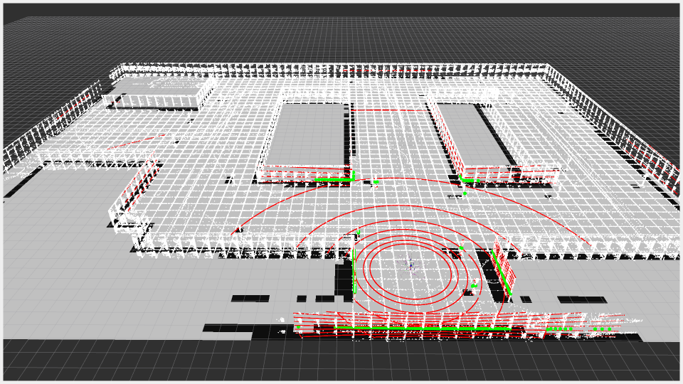
\includegraphics[width=\linewidth]{Figures/fig37.png}
    \caption{Working with a lightweight surrogate map of the environment by converting 3D LIDAR point cloud (\textcolor{red}{red}) to 2D laser scan (\textcolor{green}{green}) and applying planar mapping/localization stack for simplistic scenarios. Notice the PCD map (\textcolor{black!25}{white}) and BOG map (\textcolor{black!75}{gray}) overlaid on top of each other.}
    \label{fig: figure37}
\end{figure}

It is noteworthy to highlight that multiple high-level system configurations have been implemented within the original Autoware stack to ensure the effective operation of autonomous vehicles. Firstly, a trajectory looping criterion has been integrated to determine whether the very first waypoint in the reference trajectory should become the target waypoint for the controller upon successful tracking of the last waypoint in the reference trajectory. This feature is pivotal in shaping a "safe termination" behavior for the ego vehicle at the conclusion of the reference trajectory, particularly crucial in applications like autonomous valet parking. Additionally, the tolerance on the termination criteria is designed to enable the ego vehicle to smoothly come to a safe stop, avoiding unnecessary aggressive over-corrections or overshooting beyond the safe space. Secondly, an operational control mode has been introduced, allowing selective engagement of the ego vehicle in various modes of operation, including options of a simplistic gym environment, high-fidelity simulation environment, pure testbed (real-world hardware), or within a true digital twin framework leveraging the high-fidelity simulator in conjunction with the testbed.

Another distinctive contribution to the project lies in the creation of numerous custom meta-packages within the Autoware stack, addressing the variability in inputs, outputs, and configurations of perception, planning, and control modules across different vehicle platforms. This strategic approach ensures the project's overall cleanliness and organization. Each custom meta-package is designed to accommodate specific perception, planning, and control algorithms tailored to different vehicles within independent individual packages, thereby effectively managing diverse input and output information. Additionally, a dedicated meta-package has been established to streamline the handling of various vehicles within the AutoDRIVE Ecosystem utilized in this project, namely Nigel, F1TENTH, Hunter SE, and OpenCAV. Each individual package associated with a specific vehicle encompasses vehicle-specific parameter description configuration files for perception, planning, and control algorithms, along with map files, RViz configuration files, API program files, teleoperation program files, and user-friendly launch files, thereby ensuring a systematic and efficient management of project components.

Finally, in the case of mid and full-scale autonomous vehicles employing 3D LIDARs for exteroceptive perception of the environment, we have set up an end-to-end demonstration of converting the 3D point cloud data to a 2D laser scan datatype and operating on it for mapping and localization to aid in “lightweight” autonomous navigation (Fig. \ref{fig: figure37}). Particularly, this approach eradicates the need for utilizing complex algorithms for mapping and localization using 3D point cloud datatype. Instead, the converted 2D laser scan requiring much less computational overhead can be used with 2D mapping and localization algorithms widely adopted in the domain of autonomous mobile robots thereby reducing the computational burden from the algorithm complexity perspective as well. However, it is worth mentioning that this approach is only recommended when the environment is highly structured and loss of information from the third dimension creates little to no effect on the interpretation of environmental features based on the converted data.

\hypertarget{Challenges Faced}{%
\subsection{Challenges Faced}\label{Challenges Faced}}

\begin{figure}[t]
    \centering
    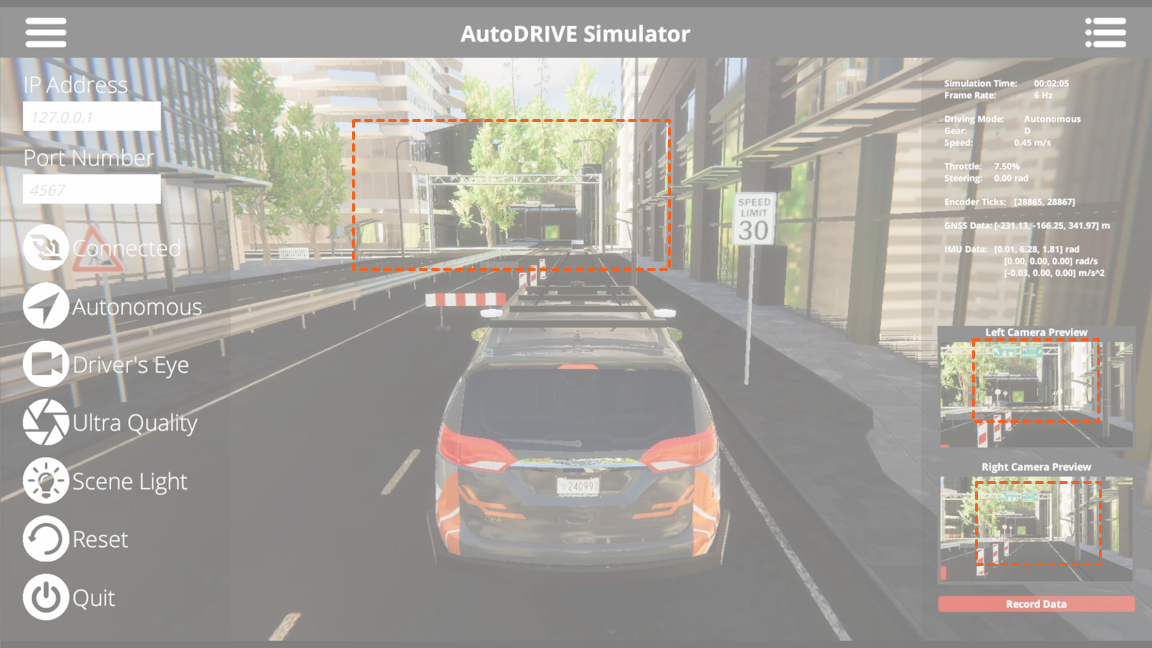
\includegraphics[width=\linewidth]{Figures/fig38.png}
    \caption{LOD culling gradually degrades the environmental details as they move further away from the scene camera. However, it does not affect any of the AV camera sensor(s). Notice the street signs at a distance culled from the scene camera, but visible in the AV camera sensor(s).}
    \label{fig: figure38}
\end{figure}

In the context of small-scale vehicles, the Autoware build process poses a significant challenge due to its prolonged duration (>8 hours) as well as its huge memory (RAM) requirement thereby impacting the efficiency of the development workflow. This problem is further aggravated since most small-scale autonomous vehicle platforms are battery-operated (with limited battery life) and therefore it is necessary to disconnect all the electrically incompatible peripherals from the onboard computer and use shore power during the installation and setup phase. Additionally, conflicts arising from different ROS distributions and parallelly sourced workspaces further complicate the integration and deployment of the Autoware stack, necessitating careful resolutions such as proper isolation of environment variables to ensure seamless operation.

For mid and full-scale vehicles, the project encounters challenges related to the management of 3D LIDAR point clouds, requiring a robust approach to handle the complexity and volume of data generated. Balancing the level of detail (LOD) in simulation versus perception is a critical consideration, introducing challenges in optimizing simulation fidelity without compromising real-world accuracy (Fig. \ref{fig: figure38}). Moreover, maneuvering in tight spaces poses a distinct challenge, demanding precise control algorithms and navigation strategies to ensure the safe and effective operation of full-scale vehicles within constrained environments. Addressing these challenges is crucial for the successful development and deployment of autonomous systems for both small and full-scale vehicles.

\hypertarget{Future Plans}{%
\subsection{Future Plans}\label{Future Plans}}

\begin{figure}[h]
     \centering
     \begin{subfigure}[b]{0.49\linewidth}
         \centering
         \includegraphics[width=\linewidth]{Fig39a.png}
         \caption{F1TENTH}
         \label{fig39a}
     \end{subfigure}
     \hfill
     \begin{subfigure}[b]{0.49\linewidth}
         \centering
         \includegraphics[width=\linewidth]{Fig39b.png}
         \caption{Nigel}
         \label{fig39b}
     \end{subfigure}
     \caption{F1TENTH and Nigel demonstrating their dynamic collision avoidance capability independent of Autoware stack. Integrating this functionality within the Autoware deployment is a future plan.}
    \label{figure39}
\end{figure}

In the future trajectory of the project, several key developments are envisioned across different scales of vehicles. For small-scale vehicles, the focus lies on advancing the capabilities through multi-agent deployment, enhancing the system's adaptability to collaborative and/or competitive scenarios. Additionally, the implementation of dynamic re-planning strategies (Fig. \ref{figure39}) is imperative to address real-time environmental changes and optimize the overall navigation efficiency (especially exploiting the redundancy in 4WD4WS Nigel by solving multi-objective optimization a.k.a. Pareto optimization problems).

Mid-scale vehicles will see a crucial step forward with the sim2real configuration and setup of the Autoware stack, ensuring a seamless transition of developed algorithms from simulation to real-world deployment. This transfer is pivotal for validating the system's performance in actual operational environments. Furthermore, dynamic re-planning remains a priority for mid-scale vehicles as well, allowing the system to respond dynamically to changing scenarios and optimize path planning strategies.

For full-scale vehicles, the sim2real configuration of Autoware stack continues to be a significant focus, emphasizing the importance of validating the system's autonomy in real-world scenarios. Dynamic re-planning remains another critical aspect for adapting to dynamic environments and ensuring the safety and efficiency of autonomous operations.

These future directions planned for expanding this project even further collectively aim to enhance the functionality, adaptability, and safety of autonomous vehicles across different scales and operational design domains whilst running the Autoware stack as an open-source medium or framework for autonomous vehicle software development.

\hypertarget{Supplemental Materials}{%
\subsection{Supplemental Materials}\label{Supplemental Materials}}

All source files including codebase, project proposal, presentation slides and technical writeups used for the completion of various aspects of the capstone project are openly available on GitHub: \href{https://github.com/Tinker-Twins/Scaled-Autonomous-Vehicles}{https://github.com/Tinker-Twins/Scaled-Autonomous-Vehicles}. We have intentionally avoided mixing the codebase for Autoware deployments within this repository for cleaner organization.

The codebase for AutoDRIVE-Autoware integration has been publicly released and is openly available on GitHub. Following is a link to our repository: \href{https://github.com/Tinker-Twins/AutoDRIVE-Autoware}{https://github.com/Tinker-Twins/AutoDRIVE-Autoware}. It is worth mentioning that this repository does not host any source files pertaining to AutoDRIVE Ecosystem itself. AutoDRIVE is openly accessible through another GitHub repository of ours: \href{https://github.com/Tinker-Twins/AutoDRIVE}{https://github.com/Tinker-Twins/AutoDRIVE}. Additionally, AutoDRIVE Ecosystem has its own GitHub Organization, which hosts additional repositories: \href{https://github.com/AutoDRIVE-Ecosystem}{https://github.com/AutoDRIVE-Ecosystem}

Although the primary aim of using Git repositories for this project was to enable version control and collaborative development, this also gave us the opportunity to document all the progress using markdown files (\texttt{README.md}). Despite challenges and scarcity of time, we invested a significant amount of time and effort in building and maintaining our repositories throughout this project. We hope that this repository will help the readers better understand our efforts, outcomes and learnings from this project and potentially serve as documentation for us (or others) when trying to explore similar approaches.